\chapter{Testes e resultados}
\label{cap:resultados}

Neste capítulo será apresentada a metodologia de testes utilizada para validar o ambiente de alta disponibilidade criado, bem como os
resultados obtidos dos testes efetuados.
A metodologia de testes deste trabalho foi fundamentada nos trabalhos de \citet{reis2009} e \citet{goncalves2009}. No primeiro trabalho, 
o autor simulou falhas de três formas, que foram através do desligamento brusco do servidor, desligamento por \textit{software} e falha de rede. 
Já no segundo trabalho, foram realizados três testes, que foram a reinicialização do servidor físico, a migração de uma máquina virtual de forma
manual, e por fim um teste com migração em tempo real (\textit{live migration}).

Neste trabalho optou-se por utilizar o teste de desligamento brusco e o desligamento por \textit{software} utilizados por \citet{reis2009}.
Já do autor \citet{goncalves2009}, utilizou-se o teste de migração em tempo real, porém adaptado para simular um agendamento de manutenção de 
\textit{hardware} ou de \textit{software}.

Os três testes descritos nas próximas seções foram efetuados no ambiente de alta disponibilidade com uma máquina virtual para fins de experimento, 
por possuírem risco de perda de dados em sua execução.
%Todavia, na Seção \ref{section:comparacaofinal} será feita a medição e a análise do período de um mês no ambiente de alta disponibilidade,
%sendo que neste ambiente estarão executando os serviços críticos definidos.

\section{Teste 1 - Desligamento físico}
%Desligamento físico (simulação falha de hardware ou eletrica): 4 vezes para medir tempo de downtime dos serviços e dos nodes (servico não crítico)

Neste teste são simuladas falhas de \textit{hardware} ou falhas elétricas nos nós do \textit{cluster}. Para isso foi feito o desligamento 
forçado do servidor, ou seja, foi pressionado o botão \textit{power} até o servidor desligar.
Com este teste pode-se validar ainda o processo de \textit{failover} dos serviços (máquinas virtuais) que estavam executando no nó que falhou, 
bem como medir o tempo de indisponibilidade dos serviços. 
%Este teste juntamente com os dois testes das próximas seções foram efetuados no 
%ambiente de alta disponibilidade com uma máquina virtual para fins de experimento, por possuírem risco de perda de dados em sua execução.

Esse teste de desligamento foi executado 4 vezes no \textit{cluster} juntamente com um \textit{script} que faz a coleta do tempo de
indisponibilidade e da latência dos dois nós e de uma máquina virtual, essa coleta é necessária para comparar os tempos de indisponibilidade da
máquina virtual e dos nós. 
Esse \textit{script} que está localizado no Apêndice \ref{ap:scriptindisp} utiliza o comando \textit{ping} para medir o tempo de indisponibilidade 
e possui um tempo de 5 minutos para sua execução. Na Tabela \ref{tab:teste1resultados} são apresentados os dados coletados desses testes efetuados. 
Pode-se observar que o tempo de indisponibilidade da máquina virtual é baixo, sendo apenas 81 segundos, pois a \ac{VM} é iniciada em um outro 
nó logo após o desligamento do primeiro nó. Essa indisponibilidade é baixa comparado com os servidores físicos que são de 169 e 205,5 segundos. 
O desvio padrão demonstra que, nos testes realizados, existe pouca variação de tempo de indisponibilidade da máquina virtual.
revisar ??

% feito em 15/09

\begin{table}[h!]
\caption{Resultados do teste de desligamento físico, contendo o tempo de indisponibilidade medido durante o teste e o desvio padrão.}
\label{tab:teste1resultados}
\begin{center}
\begin{tabular}{|l|l|l|}\hline
 & \textbf{Tempo de indisponibilidade médio} & \textbf{Desvio padrão da indisponibilidade} \\\hline
Nó 1 & 124 segundos & 4,24 \\\hline
Nó 2 & 170,5 segundos & 6,36 \\\hline
Máquina virtual & 81 segundos & 7,07 \\\hline
\end{tabular}
\end{center}
\end{table}

Destaca-se que, caso um servidor de virtualização sem esta solução de alta disponibilidade fosse reiniciado, por uma falha elétrica por exemplo, 
o tempo para reestabelecer o serviço seria igual a soma do tempo de inicialização do servidor físico mais o tempo da máquina virtual, 
que totalizaria aproximadamente 270 segundos. 
Na pior das hipóteses, caso haja uma perca definitiva do servidor físico, sendo necessário reconfigurar a máquina virtual, reinstalar as aplicações,
configurá-las e restaurar o \textit{backup}, o \ac{MTTR} seria significativamente maior. Dependendo do servidor e da aplicação, 
a indisponibilidade poderia ser maior que 24 horas.
%talvez adicionar um teste de desligamento de um servidor comum para comparar os tempos de indisponibilidade??

%O procedimento deste teste é o seguinte:
%\begin{itemize}
% \item Acessar o terminal do servidor de monitoramento;
% \item Executar comando \textit{ping} e medir o tempo de indisponibilidade (\textit{script} no Apêndice \ref{ap:scriptindisp});
% \item Forçar desligamento do nó;
% \item Aguardar máquinas virtuais inicirem no outro nó;
% \item Finalizar a medição do tempo e \textit{ping}.
%\end{itemize}

colocar em um apendice os graficos??
% A Figura \ref{fig:teste1_disponibilidade} demonstra a disponibilidade dos servidores físicos Nó 1 (\textit{Brina}) e Nó 2 (\textit{Piova}) e da 
% máquinas virtual (\textit{Trapel}). A máquina virtual teve apenas 1 minuto e 10 segundos de \textit{downtime}, deste modo, caso o 
% \textit{hardware} no qual a máquina virtual está executando falhe, o serviço será reestabelecido neste curto período de tempo.
% 
% \begin{figure}[h!]
%  \centering
%  \includegraphics[width=470px]{img/teste1_disponibilidade.eps}
%  \caption{Disponibilidade servidores físicos \textit{Brina} e \textit{Piova} e da máquina virtual \textit{Trapel}.}
%  \label{fig:teste1_disponibilidade}
% \end{figure}


\section{Teste 2 - Desligamento por software}

Esse teste simula falhas de \textit{software} nos nós do \textit{cluster}, como por exemplo, o \textit{software} de virtualização para de funcionar,
desta forma o nó não consegue iniciar a máquina virtual. Esse tipo de situação também pode ocorrer em uma manutenção emergencial, onde, 
por exemplo, é preciso desligar um servidor físico de forma emergencial. Desta forma, pode-se verificar a capacidade do outro nó manter os serviços
em funcionamento. Para simular esta situação, foram acessados os nós via \ac{SSH} e executado o comando \textit{reboot}.

% O procedimento deste teste é o seguinte:
% \begin{itemize}
%  \item Acessar o terminal do servidor de monitoramento;
%  \item Executar comando \textit{ping} e medir o tempo de indisponibilidade (\textit{script} no Apêndice \ref{ap:scriptindisp});
%  \item Acessar o terminal do nó que será reiniciado;
%  \item Executar o comando \textit{reboot};
%  \item Aguardar máquinas virtuais inicirem no outro nó e aguardar retorno do nó reiniciado;
%  \item Finalizar a medição do tempo e \textit{ping}.
% \end{itemize}

Este teste foi executado 4 vezes nos nós do \textit{cluster}. Também foi utilizado o mesmo \textit{script} utilizado no teste da Seção anterior
(Apêndice \ref{ap:scriptindisp}) para a coleta dos dados de indisponibilidade. A medição foi feita nos dois nós e também na máquina virtual, para
possibilitar a análise e comparação.
A Tabela \ref{tab:teste2resultados} demonstra o tempo de indisponibilidade e o desvio padrão dos servidores físicos e da máquina virtual.
Pode-se observar que o tempo de indisponibilidade do máquina virtual é consideravelmente menor que o tempo do servidor físico, ele representa 
apenas 3,27\% do tempo de indisponibilidade do servidor físico. 
A alguns meses ocorreu um problema semelhante a este teste, um servidor de virtualização, que é atualizado de forma automática, foi reiniciado, 
porém ocorreu um erro na atualização e o servidor não pôde iniciar corretamente. Os serviços executados nele ficaram aproximadamente 
6 horas indisponíveis.
% feito em 09/09

\begin{table}[h!]
\caption{Resultados do teste de desligamento por \textit{software}.}
\label{tab:teste2resultados}
\begin{center}
\begin{tabular}{|l|l|l|}\hline
 & \textbf{Tempo de indisponibilidade média} & \textbf{Desvio padrão da indisponibilidade} \\\hline
Nó 1 & 138,5 segundos & 2,12 \\\hline
Nó 2 & 167 segundos & 1,41 \\\hline
Máquina virtual & 10 segundos & 0 \\\hline
\end{tabular}
\end{center}
\end{table}


\section{Teste 3 - Manutenção agendada}
%Agendamento de manutenção (reboot para atualização de software): 2 semanas ou mais, 1 manutenção por semana, com live migration, reboot e 
%atualizacao de kernel dos nodes. Resultados: latencia, comparacao downtime servidor virtual e fisico, log

Reinicializações são necessárias para manutenções de \textit{hardware}, atualização de \textit{software} e até mesmo para 
rejuvenescimento\footnote{O rejuvenescimento de \textit{software} consiste na aplicações de métodos para remover problemas gerados pelo 
envelhecimento. Um exemplo de um método é o \textit{reboot} de um sistema operacional.} 
de \textit{software} \cite{melo2014}. Desta forma, criou-se esse teste para simular manutenções previamente agendadas. Para tanto, criou-se 
um \textit{script}, disponível no Apêndice \ref{ap:scriptmanutencao}, que é responsável por migrar as \acp{VM} e reiniciar o nó.

%O procedimento deste teste é o seguinte:
%\begin{itemize}
% \item Executar comando \textit{ping} e medir o tempo de indisponibilidade (\textit{script} no Apêndice \ref{ap:scriptindisp});
% \item Executar o \textit{script} que desativa o nó (comando \textit{standby}) e executa o \textit{reboot} (Apêndice \ref{ap:scriptmanutencao});
% \item Após retorno do nó executar novamente o \textit{script} anterior para retorno do nó ao \textit{cluster};
% \item Finalizar a medição do tempo e \textit{ping}.
%\end{itemize}

Este teste foi executado 2 vezes em cada nó, durante 2 semanas. Para a execução dos \textit{scripts} foi utilizada a ferramenta 
\textit{crontab} do \textit{Linux}. Os resultados são apresentados na Tabela \ref{tab:teste3resultados}.
Pode-se observar que não houve \textit{downtime} e nem perda de pacotes na máquina virtual, desta forma também não houve indisponibilidade nos 
seus serviços. Já nos nós do \textit{cluster} tem-se um tempo de indisponibilidade devido a reinicialização do servidor.
A latência baixa da máquina virtual demonstra que não há perda significante de desempenho durante a migração da máquina virtual de um nó para outro.

% feito em 17/09 a 30/09
% crontab brina:
% */10 04 * * 2 /usr/local/sbin/script_pacemaker_manutencao.sh
% crontab piova:
% */10 04 * * 4 /usr/local/sbin/script_pacemaker_manutencao.sh
% crontab monit:
%59 03 * * 2 cd /home/bruno/pacemaker/teste2/; bash indisponibilidade.sh 186.195.16.14 1
%59 03 * * 2 cd /home/bruno/pacemaker/teste2/; bash indisponibilidade.sh 186.195.16.13 1
%59 03 * * 4 cd /home/bruno/pacemaker/teste2/; bash indisponibilidade.sh 186.195.16.6 2
%59 03 * * 4 cd /home/bruno/pacemaker/teste2/; bash indisponibilidade.sh 186.195.16.13 2

\begin{table}[h!]
\caption{Resultados do teste 3.}
\label{tab:teste3resultados}
\begin{center}
\begin{tabular}{|l|p{4cm}|p{4cm}|l|}\hline
 & \textbf{Média do tempo de indisponibilidade} & \textbf{Desvio padrão da indisponibilidade} & \textbf{Latência média} \\\hline
Nó 1 & 145,5 segundos & 0,70 & 22,63 ms \\\hline
Nó 2 & 173 segundos & 1,41 & 19,8 ms \\\hline
Máquina virtual & 0 segundos & 0 & 0,309 ms \\\hline
\end{tabular}
\end{center}
\end{table}

A Figura \ref{fig:teste2_trapel1} demonstra a disponibilidade da máquina virtual, onde pode-se perceber que não houve nenhuma indisponibilidade. 
Esses dados foram produzidos pela ferramenta \textit{Nagios} \cite{nagios}, que faz o monitoramento da empresa. 
%grafico comparativo nagios da disponibilidade do servidor fisico e do virtual
%grafico nagios - Trends(grafico) ou Availability (resumo) - Hosts - servidor - tempo 18/09 a 30/09 + Include Soft States = yes
\begin{figure}[h!]
 \centering
 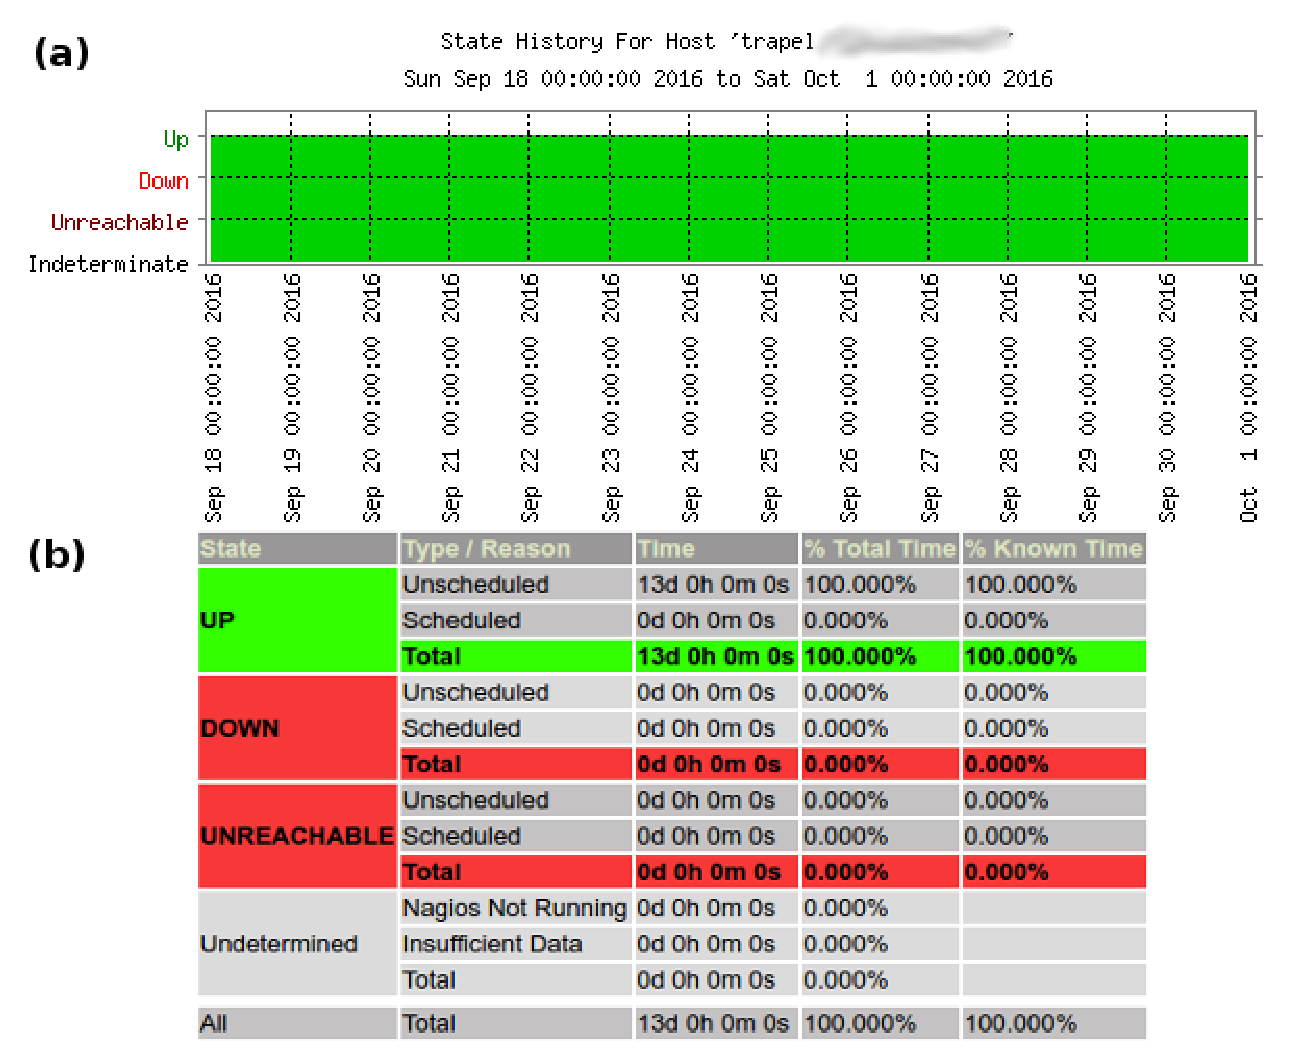
\includegraphics[width=360px]{img/teste2_trapel1.eps}
 \caption{Disponibilidade da máquina virtual, com o gráfico da disponibilidade (a) e a tabela com detalhes de tempo e percentual (b).}
 \label{fig:teste2_trapel1}
\end{figure}

Comparando os resultados da máquina virtual (Figura \ref{fig:teste2_trapel1} (b)) com os resultados dos nós 1 e 2 (Figura \ref{fig:teste2_brina1} 
(b) e Figura \ref{fig:teste2_piova1} (b)), pode-se perceber a diferença do \textit{uptime}, que fica entre 99,975\% e 99,976\% para os nós e 
100\% para a máquina virtual. Já nos gráficos da Figura \ref{fig:teste2_brina1} (a) e da Figura \ref{fig:teste2_piova1} (a), pode-se observar 
as duas reinicializações feitas.
\begin{figure}[h!]
 \centering
 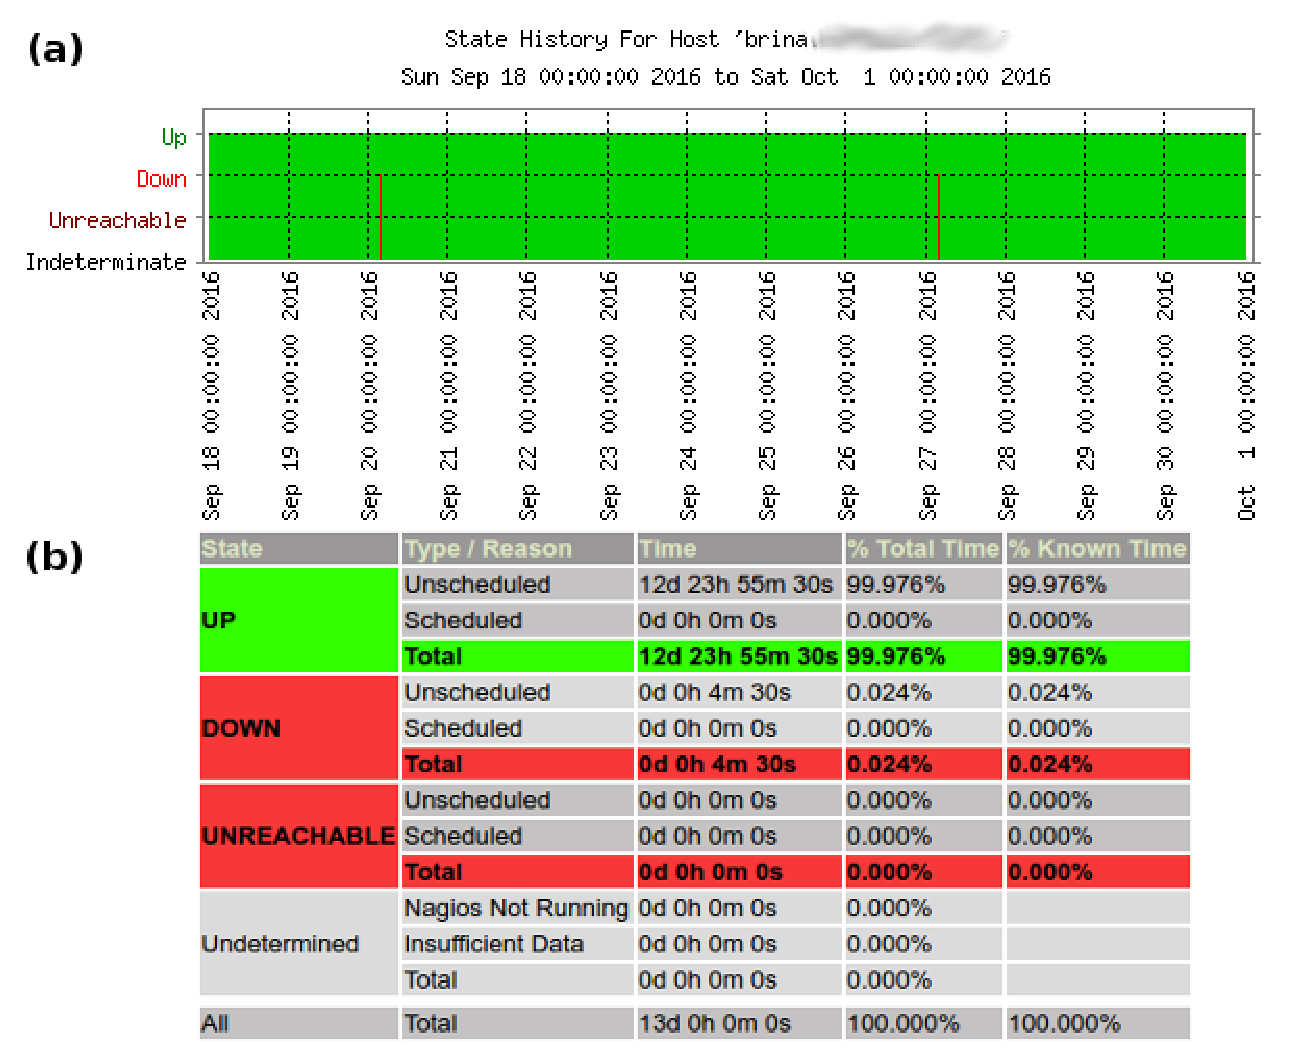
\includegraphics[width=360px]{img/teste2_brina1.eps}
 \caption{Disponibilidade do Nó 1, com o gráfico da disponibilidade (a) e a tabela com detalhes de tempo e percentual (b).}
 \label{fig:teste2_brina1}
\end{figure}

\begin{figure}[h!]
 \centering
 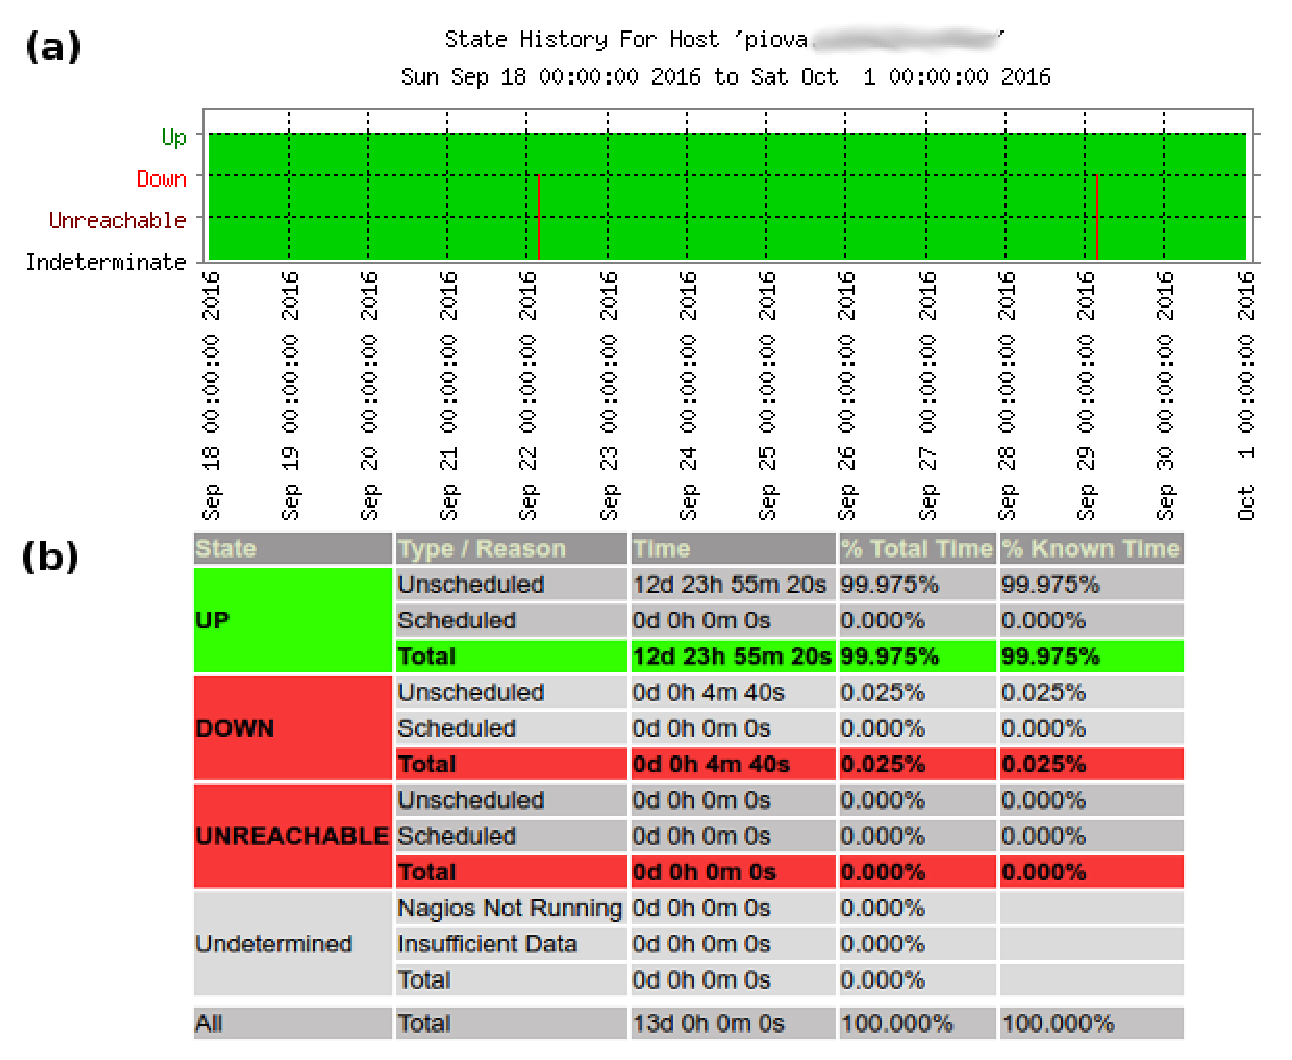
\includegraphics[width=360px]{img/teste2_piova1.eps}
 \caption{Disponibilidade do Nó 2, com o gráfico da disponibilidade (a) e a tabela com detalhes de tempo e percentual (b).}
 \label{fig:teste2_piova1}
\end{figure}

Durante o processo de \textit{live migration} a latência da máquina virtual aumentou, isso pode ser observado na Figura 
\ref{fig:teste2_latencia} através do pico ocorrido entre o tempo 50 e 100 do eixo x.
%teste2/186.195.16.13-stat-1.log
%teste2/186.195.16.13-stat-2.log
\begin{figure}[h!]
 \centering
 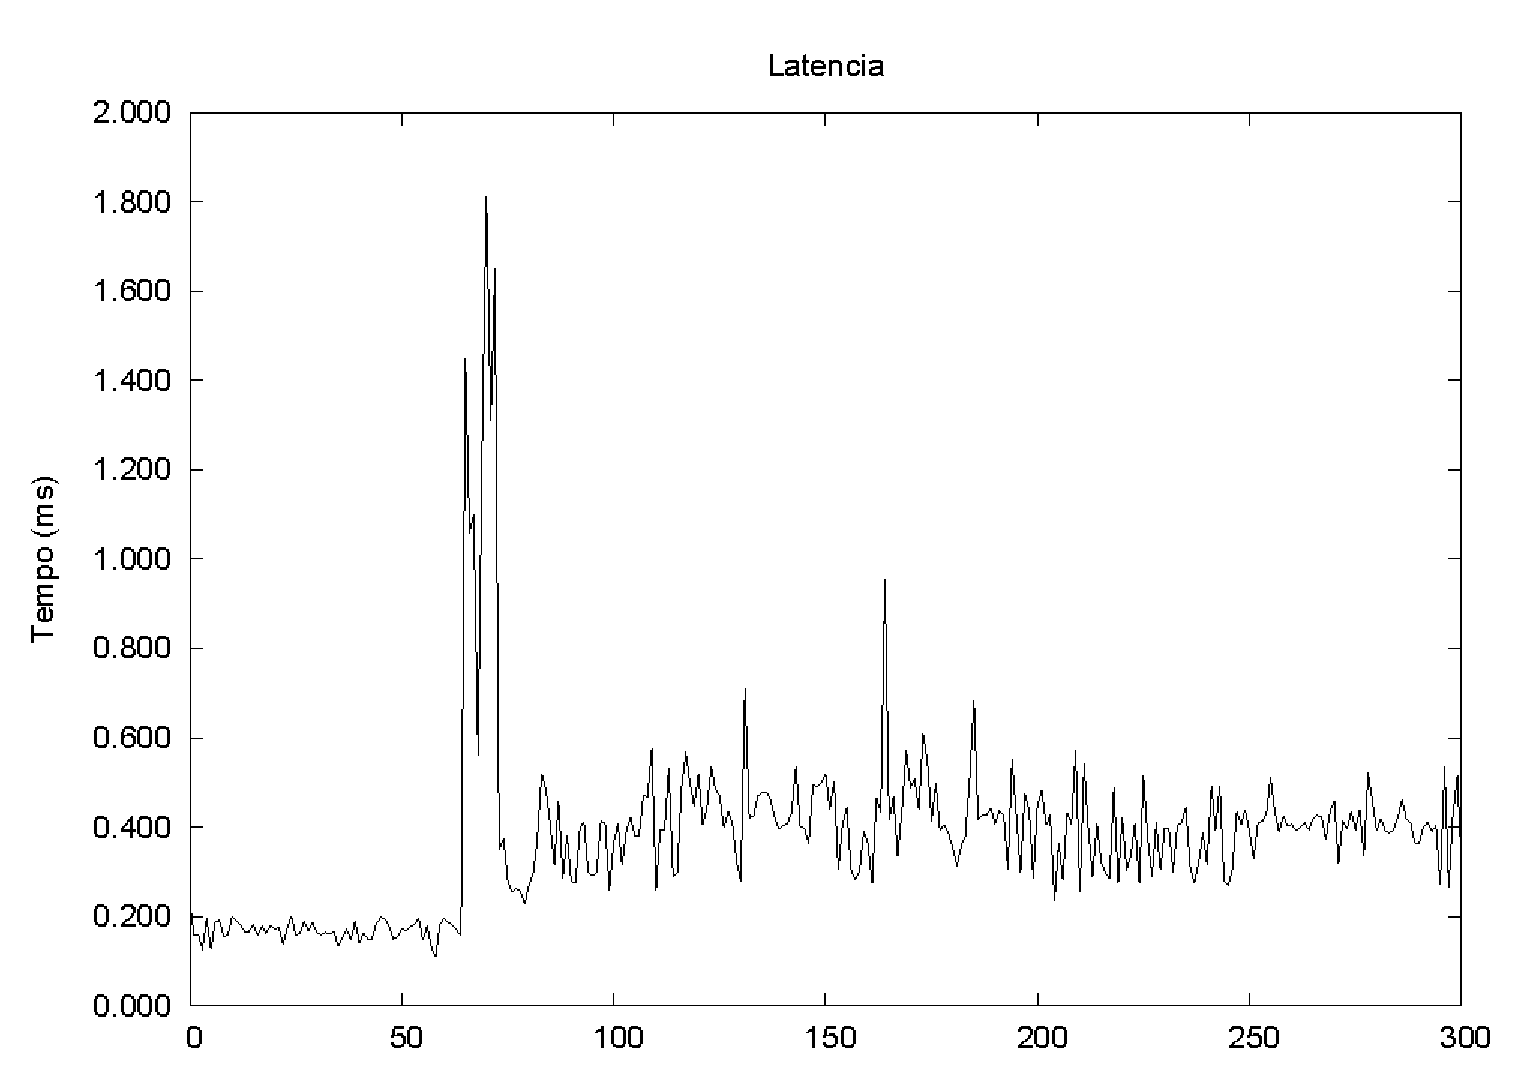
\includegraphics[width=320px]{img/teste2_latencia.eps}
 \caption{Latência da máquina virtual durante o \textit{live migration}.}
 \label{fig:teste2_latencia}
\end{figure}

%log do pacemaker
%O processo de \textit{standby} feito pelo \textit{Pacemaker} está detalhado no \textit{log} abaixo:


\subsection{Comparação final da disponibilidade}
\label{section:comparacaofinal}
%Medição da disponibilidade dos serviços críticos por 30 dias (14/10 a 12/11) FAZER uma manutencao de hardware.
%Comparar ao mês de setembro (01/09 a 30/09) no ambiente antigo com uma reinicialização dos servidores físicos (reiniciados em 06/09/16)

Nesta seção será feita a medição e a análise do período de um mês no ambiente de alta disponibilidade, sendo que neste ambiente estarão executando 
os serviços críticos definidos na Seção \ref{section:maqservcrit}.
Durante esse período foi feito uma manutenção...
%...foi mensurado a disponibilidade

... ??

adicionar gráficos de disponibilidade final dos serviços críticos:

%Medição através do comando ping e do Nagios, que utiliza ping para calcular o tempo de downtime
%Tabela com perda de pacotes, latencia, tempo de indisponibilidade X node fisico e maquina virtual


\section{Considerações finais}

Neste capítulo foi feita a análise do ambiente de alta disponibilidade implementado na empresa, através de testes e da coleta de dados
provenientes desses testes. Pode-se perceber resultados obtidos foram positivos, e que os objetivos deste trabalho foram alcançados. 
...
